\chapter{Carcasa}

La carcasa es la parte visible del producto, es la primera impresión que se lleva el usuario y, por tanto, es una parte muy importante del diseño. En este capítulo se describirá el proceso de diseño y fabricación de la carcasa del producto. Se describirán las medidas físicas, la ergonomía y el proceso de fabricación. Como se diseñó en el capítulo \ref{CapDiseño}, esta será una única pieza de madera que se fabricara con una máquina \gls{CNC}.

El plano que se utilizó para el diseño de la carcasa se creara con la herramienta AutoCAD para seguir con la decisión de la sección \ref{Herramientas}, se exportara a FreeCAD para crear el modelo 3D y se exportara a G-Code para la fabricación con la máquina \gls{CNC}.

\section{Diseño físico}
Para el diseño de la carcasa nos vamos a basar en el plano que ya tenemos de la \gls{PCB}, ya que en la sección \ref{MedidasFisicas} se dispusieron los agujeros donde iban a ir los tornillos de la misma. Se va a diseñar una carcasa que sea tipo cajón, donde la \gls{PCB} se va a deslizar por la parte superior y se va a atornillar a la parte inferior. Se va a dejar un espacio para la batería de la \gls{PCB}. Para empezar con el diseño importaremos el plano de la \gls{PCB} a AutoCAD y se creará la carcasa alrededor de la \gls{PCB}. Los bordes de la carcasa se van a redondear para darle un aspecto más estético. Además, tendrán un grosor de 7 mm para darle resistencia y poder atornillar el conector XS-12.

También se tendrá en cuenta el espacio acordado de margen de error en la figura \ref{fig:PlanoSeparacionMadera} para que la \gls{PCB} pueda deslizarse sin problemas, teniendo en cuenta errores de precisión en la fabricación de la carcasa y la \gls{PCB}. El plano final que nos queda se puede ver en la figura \ref{fig:PlanoCarcasa}.

\begin{figure}[H]
    \centering
    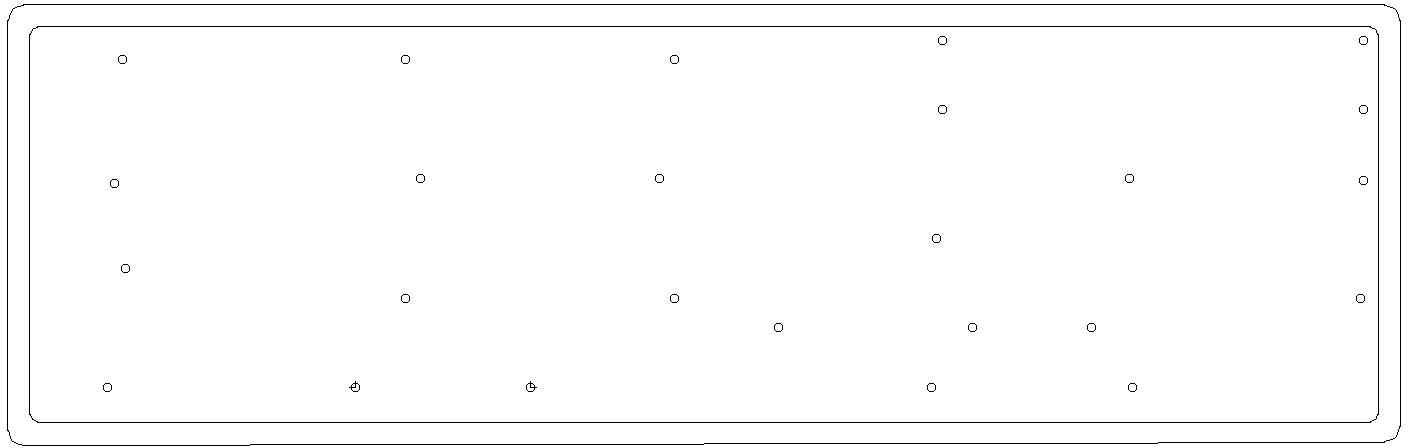
\includegraphics[width=1\textwidth]{imagenes/Capitulos/Cap06/PlanoCarcasa.png}
    \caption{Imagen del plano de la carcasa del teclado.}
    \label{fig:PlanoCarcasa}
\end{figure}

\subsection{Medidas Físicas}
A partir del plano de la figura \ref{fig:PlanoCarcasa} se va a realizar el modelo 3D de la carcasa. Para ello vamos a usar FreeCAD y vamos a extrudir las diferentes partes del plano.

Para conocer las dimensiones de la extrusión se van a crear las diferentes vistas de la carcasa y todos sus elementos.

Tras realizar las diferentes vistas ya sabemos las dimensiones exactas para crear la pieza 3D. El resultado final se puede ver en la figura \ref{fig:Modelo3D}. Si añadimos el hueco para el conector XS-12 y renderizamos el modelo con una textura de madera podemos tener una idea de como será la carcasa una vez terminada este renderizado lo podemos ver en la figura \ref{fig:Modelo3DRender}.

\begin{figure}[H]
    \centering
    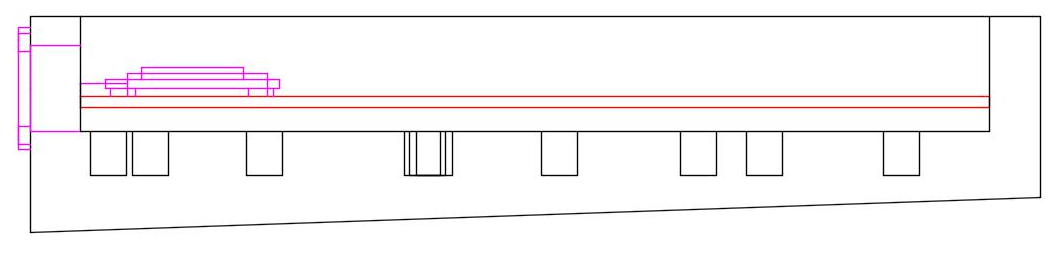
\includegraphics[width=1\textwidth]{imagenes/Capitulos/Cap06/PlanoCarcasaVistaLateral.png}
    \caption{Imagen del plano lateral (Vista perfil izquierda) de la carcasa del teclado.}
    \label{fig:PlanoCarcasaVistaLateral}
\end{figure}

\begin{figure}[H]
    \centering
    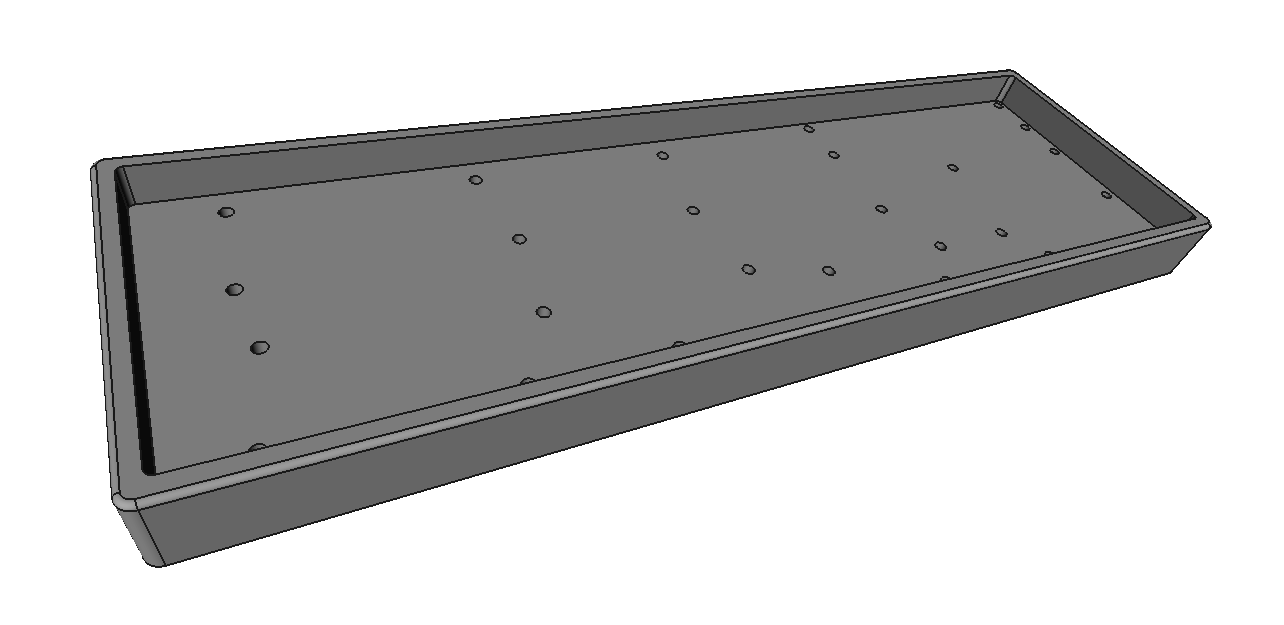
\includegraphics[width=1\textwidth]{imagenes/Capitulos/Cap06/Modelo3D.png}
    \caption{Imagen del modelo 3D de la carcasa del teclado.}
    \label{fig:Modelo3D}
\end{figure}

\begin{figure}[H]
    \centering
    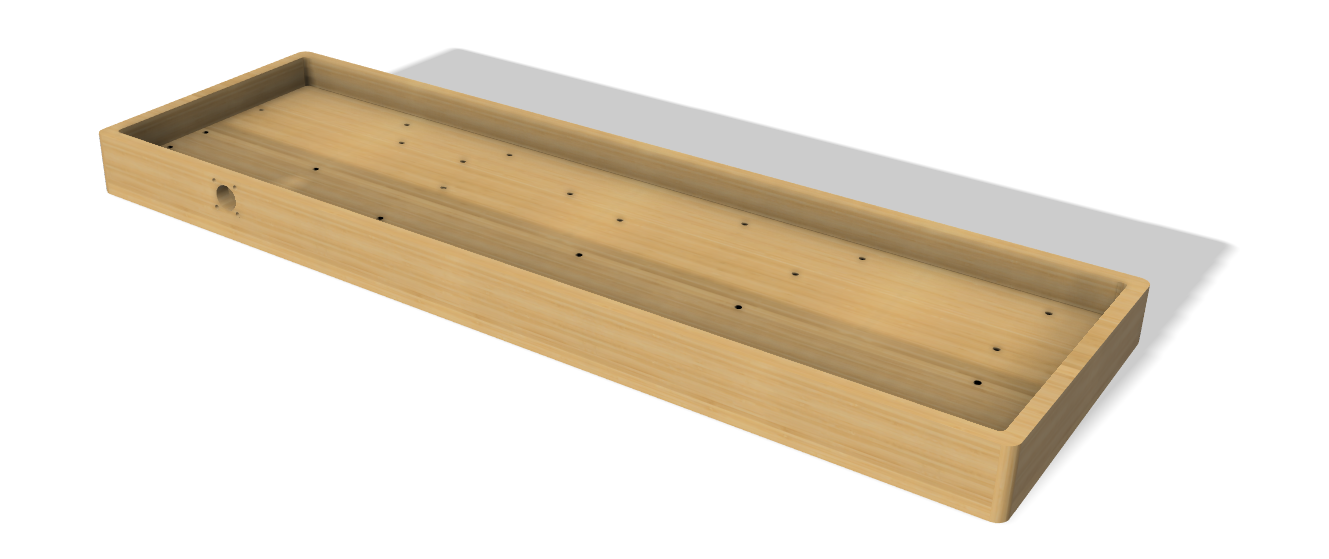
\includegraphics[width=1\textwidth]{imagenes/Capitulos/Cap06/Modelo3DRender.png}
    \caption{Imagen del modelo 3D Renderizado de la carcasa del teclado.}
    \label{fig:Modelo3DRender}
\end{figure}

\subsection{Ergonomía}
Para la ergonomía de la carcasa se ha tenido en cuenta la altura de la misma. Se ha decidido que la altura e inclinación de la carcasa sea de 2.5º para que el usuario pueda escribir de forma más cómoda. La altura de la carcasa es de 3 cm en la parte trasera y 2,5 cm en la parte delantera. La inclinación de la carcasa se puede ver en la figura \ref{fig:PlanoCarcasaVistaLateral}.

Para realizar la inclinación se hará cortando con ángulo la parte inferior una vez terminado el fresado de la carcasa. Una vez terminado se procederá a lijar la carcasa para que quede con un acabado más fino.

Una vez terminado el fresado y el lijado se procederá a barnizar la carcasa para darle un acabado más profesional y resistente a la humedad y al uso.

\section{Fabricación}
Para la fabricación de la carcasa del producto, se seguirá un proceso detallado que garantice la precisión y calidad del resultado final. Este proceso constará de varias etapas, desde la preparación de los materiales hasta el acabado final de la carcasa. A continuación se detallan las etapas de fabricación.

\subsubsection{Preparación de materiales}
Antes de iniciar el proceso de fabricación, es crucial asegurarse de tener todos los materiales necesarios en las cantidades adecuadas. Para la carcasa del producto, se requerirá una lámina de madera del tipo y grosor especificado en el diseño, así como los dispositivos de sujeción necesarios para fijar la madera durante el proceso de fresado. También se necesitará un barniz protector para el acabado final de la carcasa. Los tornillos de empotrado y un fijador como bien puede ser epoxi para fijar los tornillos a la carcasa.

\subsubsection{Programación de la máquina CNC}
Una vez asegurados los materiales, se procederá a programar la máquina CNC con el código G generado a partir del modelo 3D de la carcasa. Este código instruirá a la máquina sobre los movimientos necesarios para esculpir la forma deseada en la lámina de madera. Se verificará cuidadosamente que el código esté libre de errores y que refleje fielmente el diseño de la carcasa.

\subsubsection{Fresado de la carcasa}
Con la máquina CNC debidamente programada, se llevará a cabo el fresado de la carcasa en la lámina de madera. Durante este proceso, se prestará especial atención para garantizar la precisión en cada paso, asegurando que las dimensiones y formas coincidan con las especificaciones del diseño. Se realizarán las operaciones de fresado necesarias para crear los contornos, agujeros y detalles requeridos en la carcasa.

\subsubsection{Corte con ángulo y lijado}
Una vez completado el fresado, se procederá al corte con ángulo en la parte inferior de la carcasa para darle la inclinación deseada. Este paso se realizará con una sierra de banco con medidor de ángulo para garantizar la precisión en el corte. Posteriormente, se lijará la carcasa para eliminar cualquier imperfección y suavizar las superficies. Se utilizarán lijas de grano fino para poder aplicar el barniz de forma uniforme y obtener un acabado suave.

\subsubsection{Atornillado}
Una vez lijada la carcasa, se procederá a atornillar las tuercas hexagonales para inserción en muebles. Estas tuercas se atornillarán en los agujeros de la carcasa para fijar la PCB y el conector XS-12. Se utilizará un fijador como epoxi para asegurar que las tuercas queden firmemente sujetas a la madera. Se verificará que las tuercas estén alineadas correctamente y que los tornillos de la PCB y el conector XS-12 encajen de forma segura. Una vez completado el atornillado se taparán los agujeros internos con un tornillo o utilizando un tapón para evitar que el barniz entre en ellos.

\subsubsection{Acabado final}
Finalmente, se aplicará un barniz protector a la carcasa para proporcionarle un acabado profesional y resistente. Este barniz no solo mejorará la apariencia estética de la carcasa, sino que también la protegerá contra la humedad y el desgaste durante el uso. Se dejará secar el barniz según las instrucciones del fabricante. Una vez seco, se inspeccionará la carcasa para asegurarse de que el acabado sea uniforme y de alta calidad.